% Compatibility with a newer local hyperref on a pre-metadata LaTeX kernel.
\providecommand\IfDocumentMetadataT[1]{}
\documentclass[aspectratio=169,11pt]{beamer}
\usepackage[T1]{fontenc}
\usepackage[utf8]{inputenc}
\usepackage{lmodern}
\usepackage{amsmath,amssymb,booktabs,graphicx,listings,tikz}
\usetikzlibrary{arrows.meta,positioning,calc}
\definecolor{ink}{HTML}{122838}
\definecolor{teal}{HTML}{007F76}
\definecolor{mint}{HTML}{65D4C1}
\definecolor{rust}{HTML}{A25728}
\definecolor{muted}{HTML}{536C7A}
\definecolor{wash}{HTML}{EDF5F4}
\definecolor{hairline}{HTML}{DCE6E9}
\setbeamercolor{normal text}{fg=ink,bg=white}
\setbeamercolor{structure}{fg=teal}
\setbeamercolor{frametitle}{fg=ink}
\setbeamercolor{alerted text}{fg=rust}
\setbeamertemplate{navigation symbols}{}
\setbeamertemplate{itemize item}{\color{teal}\raisebox{.15ex}{\tiny$\blacksquare$}}
\setbeamersize{text margin left=9mm,text margin right=9mm}
\setbeamerfont{frametitle}{size=\Large,series=\bfseries}
\newcommand{\chaptertag}{01\quad THE ECONOMICS}
\setbeamertemplate{headline}{\vspace{2mm}\hspace{9mm}{\color{teal}\fontsize{7}{8}\selectfont\bfseries\chaptertag}\vspace{1mm}}
\setbeamertemplate{frametitle}{\vspace{1mm}\insertframetitle\par\vspace{2mm}{\color{hairline}\hrule}\vspace{1mm}}
\setbeamertemplate{footline}{\hspace{9mm}{\color{muted}\fontsize{6.7}{8}\selectfont IDE \& TALAM\`AS (2025)\hfill ECONOMICS $\to$ LEAN\hspace{6mm}\insertframenumber\hspace{9mm}}\vspace{3mm}}
\newcommand{\src}[1]{\vfill\vspace{0mm}{\fontsize{6.8}{8}\selectfont\color{muted}#1\par}}
\newcommand{\take}[1]{\par\vspace{1mm}\noindent\colorbox{wash}{\parbox{\dimexpr\linewidth-2\fboxsep}{\vspace{1mm}\color{ink}\small\raggedright #1\vspace{1mm}}}}
\newcommand{\labeltext}[1]{{\color{teal}\small\bfseries #1}\par\vspace{2mm}}
\newcommand{\bigstat}[2]{{\color{teal}\fontsize{27}{30}\selectfont\bfseries #1}\par\vspace{1mm}{\small #2}}
\newcommand{\wa}{w^{A}}
\newcommand{\wn}{w^{N}}
\renewcommand{\arraystretch}{1.25}
\lstdefinelanguage{Lean}{morekeywords={def,theorem,by,have,intro,unfold,noncomputable,calc,using},sensitive=true,morecomment=[l]{--}}
\lstset{language=Lean,basicstyle=\ttfamily\footnotesize,breaklines=true,columns=fullflexible,keepspaces=true,showstringspaces=false,keywordstyle=\bfseries\color{teal},commentstyle=\color{muted},backgroundcolor=\color{wash},frame=none,aboveskip=3pt,belowskip=3pt,xleftmargin=3pt,xrightmargin=3pt,framexleftmargin=3pt,literate={ℝ}{{$\mathbb R$}}1 {∀}{{$\forall$}}1 {→}{{$\to$}}1 {≤}{{$\le$}}1 {≠}{{$\ne$}}1 {↔}{{$\leftrightarrow$}}1 {₀}{{$_0$}}1}
\pdfstringdefDisableCommands{\def\\{ }\def\translate#1{#1}}

\hypersetup{pdftitle={AI in the knowledge economy: autonomy, capability, and proof},pdfauthor={Ide and Talamas (2025); weekly presentation}}
\begin{document}

% 01 — 0:24
{\setbeamercolor{background canvas}{bg=ink}
\begin{frame}[plain]
\vspace{3mm}
{\color{mint}\small\bfseries ECONOMIC MODELING $\times$ FORMAL VERIFICATION}\par
\vspace{7mm}
{\color{white}\fontsize{31}{35}\selectfont\bfseries Who gains\\from AI?}\par
\vspace{4mm}
{\color{mint}\Large Autonomy. Capability. Proof.}\par
\vspace{5mm}
{\color{white}\normalsize Ide \& Talam\`as (2025)}\par
\vfill
{\color{white}\small\href{https://github.com/gsaco/ai-05-ide}{github.com/gsaco/ai-05-ide}}\par
\vspace{3mm}
{\color{white!65}\scriptsize Read: course PDF, May 20, 2025 (39 pp).\quad Lean pin: arXiv v11, February 25, 2025 (35 pp).}
\end{frame}}

\begin{frame}{Two dimensions. Three outcomes.}
\begin{columns}[T,onlytextwidth]
\begin{column}{.48\textwidth}
\labeltext{AUTONOMY = PERMITTED ROLES}
\textbf{Autonomous AI}\\[2mm]
Produces, works, and advises.\\[4mm]
\textbf{Co-pilot-only AI}\\[2mm]
Advises; cannot initiate production.
\end{column}
\begin{column}{.48\textwidth}
\labeltext{CAPABILITY = KNOWLEDGE}
\[a=z_{AI}\in[0,1).\]
The fraction of problems AI can solve.\\[4mm]
A permitted role may still be unprofitable.
\end{column}
\end{columns}
\take{Track \textbf{bottom wages}, \textbf{top wages}, and \textbf{total output}. The sign cannot be inferred from autonomy alone.}
\src{Today: source claims $\to$ a three-type economy $\to$ seven slides on what Lean checks.}
\end{frame}

\begin{frame}{Knowledge helps only when someone supplies time}
\centering
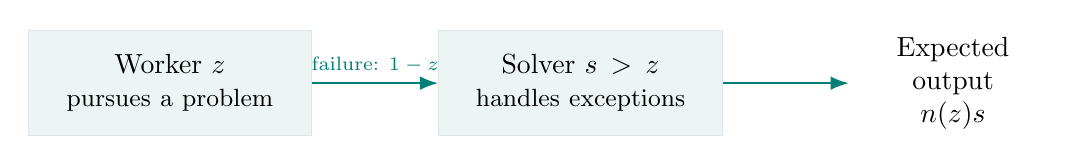
\begin{tikzpicture}[>=Latex,node distance=16mm]
\node[draw=hairline,fill=wash,text width=30mm,align=center,inner sep=3mm] (w) {Worker $z$\\\small pursues a problem};
\node[right=of w,draw=hairline,fill=wash,text width=30mm,align=center,inner sep=3mm] (s) {Solver $s>z$\\\small handles exceptions};
\node[right=of s,text width=24mm,align=center] (o) {Expected output\\$n(z)s$};
\draw[->,thick,teal] (w)--node[above,font=\scriptsize] {failure: $1-z$}(s);
\draw[->,thick,teal] (s)--(o);
\end{tikzpicture}
\[
h\,n(z)(1-z)=1
\quad\Longrightarrow\quad n(z)=\frac{1}{h(1-z)}.
\]
\[
\max_{\text{organization},\,z,s}\Pi,
\qquad \Pi_{HH}=n(z)[s-w(z)]-w(s).
\]
\small Humans maximize income; firms choose teams; competitive entry sets active profits to zero. Labor and compute markets clear.
\src{Section 3.1. Difficulty is uniform on $[0,1]$; each request costs $h$ solver time, successful or not.}
\end{frame}

\begin{frame}{Keep the conditions attached to the result}
\begin{columns}[T,onlytextwidth]
\begin{column}{.49\textwidth}
\labeltext{PEOPLE AND FIRMS}
\small Unit human mass; one unit of time each. Observable knowledge $z\in[0,1]$ with continuous, strictly positive density.\\[3mm]
Independent uniform difficulties; risk neutrality; output price one. Competition, complete information, no fixed costs; at most two layers.
\end{column}
\begin{column}{.46\textwidth}
\labeltext{TECHNOLOGY AND SCARCITY}
\small $0<h<h_0$: no independent humans before AI.\\[3mm]
$a<1$: perfect AI is excluded.\\[3mm]
Compute abundant relative to human time; opportunities exceed production capacity.\\[3mm]
Compare autonomy at the same $a$ and $\mu$.
\end{column}
\end{columns}
\take{The source's top-winner result needs \textbf{both $h<h_0$ and $a<1$}. The appendix gives the sufficient compute bound.}
\src{Sections 3.1, 3.3, 5.2 and 6. These continuum assumptions are not inherited by the finite example.}
\end{frame}

\begin{frame}{Proposition 5: capability creates bottom winners}
\begin{columns}[T,onlytextwidth]
\begin{column}{.59\textwidth}
\labeltext{BOTTOM: A STRICT THRESHOLD}
\[
B\ne\varnothing\quad\Longleftrightarrow\quad a>\bar a,
\qquad\bar a\in\operatorname{int}W.
\]
\small $W$: the pre-AI worker set. $B$: humans below AI who earn more than before.\\[3mm]
The threshold lies \emph{inside} the worker region: some ``basic'' AI already benefits the bottom.
\end{column}
\begin{column}{.35\textwidth}
\labeltext{TOP: ALWAYS SOME WINNERS}
\[T\ne\varnothing\quad\forall a\in[0,1).\]
\small Under the stated conditions, some humans above AI gain.\\[3mm]
The human with knowledge $a$ loses.
\end{column}
\end{columns}
\take{Autonomy is held fixed in this proposition. \textbf{Capability still changes the distributional conclusion.}}
\src{$B=\{z\le a:\wa(z)>w(z)\}$, $T=\{z\ge a:\wa(z)>w(z)\}$ within $[0,1]$. v11 p.24 / course p.25.}
\end{frame}

\begin{frame}{Proposition 6: free advice must still be useful}
\begin{center}\small
\begin{tabular}{p{30mm}p{90mm}}
\toprule
\textbf{Capability} & \textbf{Co-pilot-only equilibrium, $r^N=0$}\\
\midrule
$a\le w(0)$ & No adoption. Wages and occupations unchanged.\\
$a>w(0)$ & Lowest-knowledge humans adopt. Strict bottom gains and some strict human losses.\\
\bottomrule
\end{tabular}\end{center}
\vspace{2mm}
\begin{columns}[T,onlytextwidth]
\begin{column}{.31\textwidth}\labeltext{NEAR THE BOTTOM}\small $\wn\ge\max\{w,\wa\}$; strict if $a>w(0)$.\end{column}
\begin{column}{.31\textwidth}\labeltext{NEAR THE TOP}\small $\wn\le\wa$; strict away from $z=1$.\end{column}
\begin{column}{.31\textwidth}\labeltext{TOTAL OUTPUT}\small $Y^A>Y^N$. Efficiency is relative to the permitted technology.\end{column}
\end{columns}
\take{$w(0)$ is an \textbf{adoption threshold}; $\bar a$ is an \textbf{autonomous bottom-gain threshold}. They are distinct.}
\src{v11 p.27 / course p.28. Complete quantifiers, uniqueness and occupational clauses: appendix.}
\end{frame}

\renewcommand{\chaptertag}{02\quad THE THREE-TYPE CHECK}
\begin{frame}{Three types make the wage equations tangible}
\begin{columns}[T,onlytextwidth]
\begin{column}{.39\textwidth}
\labeltext{OUR FINITE ECONOMY}
\begin{tabular}{lrr}\toprule
Type & $z$ & Mass\\\midrule
Low & $0$ & $.55$\\
Middle & $1/2$ & $.30$\\
High & $1$ & $.15$\\\bottomrule
\end{tabular}\\[3mm]
$h=1/2,\quad\mu=2$.
\end{column}
\begin{column}{.55\textwidth}
\labeltext{ZERO PROFIT BEFORE AI}
\[
u+\tfrac12v=\tfrac12,\quad u+\tfrac12t=1,\quad v+\tfrac14t=1.
\]
Subtract the first two: $t-v=1$. Then
\[\boxed{(u,v,t)=(.2,.6,1.6)}.\]
\small Worker masses $(L\to M,L\to H,M\to H)$\\are $(.32,.23,.14)$; all resources clear.
\end{column}
\end{columns}
\take{The finite economy is derived directly. It changes the source's continuous-density assumption.}
\src{Complete resource equations and no-entry checks: analysis/derivation.md. Baseline output $Y_0=.53$.}
\end{frame}

\begin{frame}{Autonomous AI pins wages through outside options}
\labeltext{DERIVED BRANCH: $0<a<1/3$; SPARE COMPUTE PINS $r^A=a$}
\begin{center}
\begin{tabular}{p{66mm}l}\toprule
\textbf{Active human role} & \textbf{Competitive wage}\\\midrule
High: supervise AI workers & $t=(1-a)/[(1-a)/2]=2$\\[3mm]
Middle: supervise AI workers & $v=(1-2a)/(1-a)$\\[3mm]
Low: work with middle solvers & $u=\frac12-\frac12v=a/[2(1-a)]$\\\bottomrule
\end{tabular}
\end{center}
\take{$.55$ low workers use $.275$ middle solvers. The remaining $.025$ middle humans supervise AI, pinning $v$.}
\src{AI-worker compute use $7/[20(1-a)]<2$; spare compute and all no-entry inequalities checked.}
\end{frame}

\begin{frame}{Same autonomy; the bottom changes from loss to gain}
\[
\frac{a}{2(1-a)}>\frac15
\quad\Longleftrightarrow\quad 5a>2(1-a)
\quad\Longleftrightarrow\quad \boxed{a>\frac27}.
\]
\centering
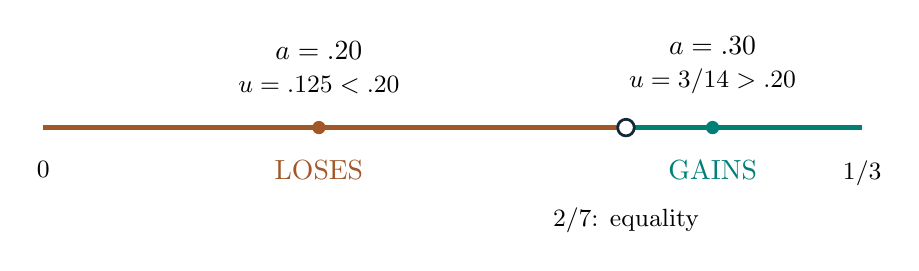
\begin{tikzpicture}[x=1cm,y=1cm]
\draw[line width=2pt,rust] (0,0)--(7.4,0);
\draw[line width=2pt,teal] (7.4,0)--(10.4,0);
\fill[rust] (3.5,0) circle(2.4pt);\fill[teal] (8.5,0) circle(2.4pt);
\draw[ink,fill=white,line width=1pt] (7.4,0) circle(3pt);
\node[above=3mm,align=center] at(3.5,0){$a=.20$\\\small $u=.125<.20$};
\node[above=3mm,align=center] at(8.5,0){$a=.30$\\\small $u=3/14>.20$};
\node[below=3mm,rust] at(3.5,0){LOSES};
\node[below=3mm,teal] at(8.5,0){GAINS};
\node[below=9mm,font=\small] at(7.4,0){$2/7$: equality};
\node[below=3mm,font=\small] at(0,0){$0$};
\node[below=3mm,font=\small] at(10.4,0){$1/3$};
\end{tikzpicture}
\take{The denominator is positive. At $a=2/7$ there is \emph{no strict gain}. Lean will check exactly this inequality and its domain.}
\src{Schematic line; positions are illustrative. $2/7$ is our finite-branch threshold, not the continuum's numerical cutoff.}
\end{frame}

\begin{frame}{The numerical check captures both dimensions}
\centering
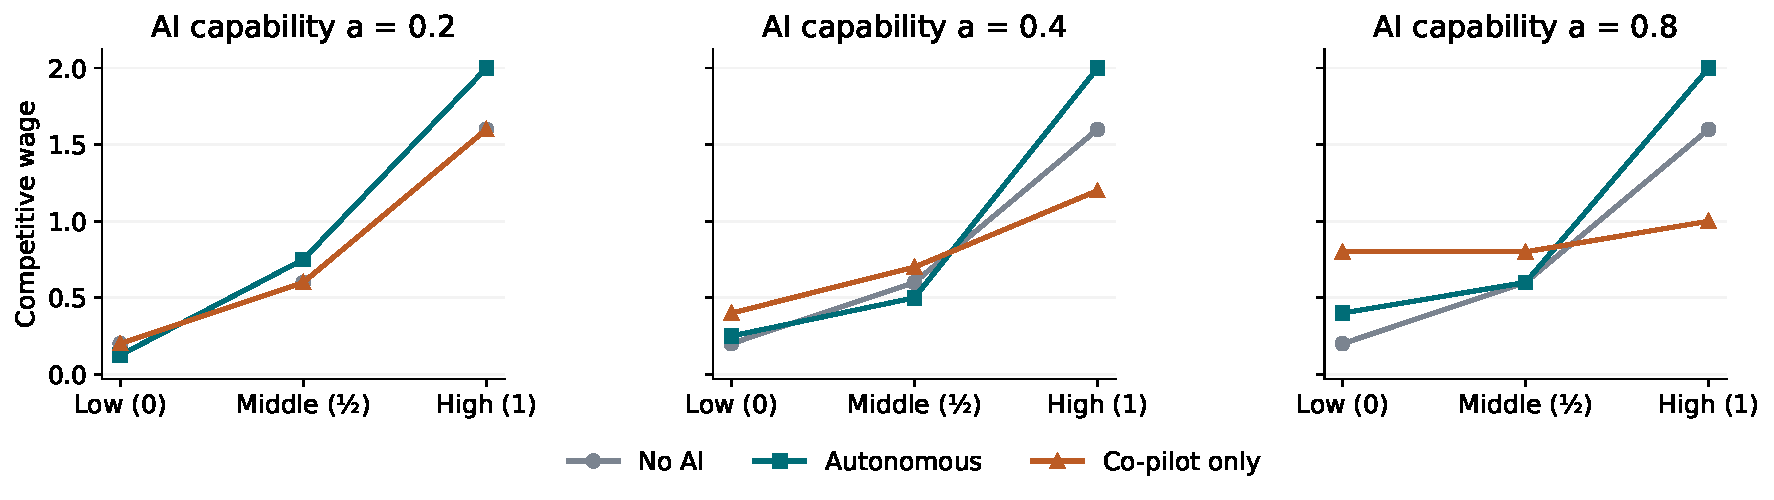
\includegraphics[width=\textwidth,height=.57\textheight,keepaspectratio]{figures/discrete_wages.pdf}
\vspace{2mm}
\begin{columns}[T,onlytextwidth]
\begin{column}{.48\textwidth}\small\textbf{Read across panels:} change capability while holding autonomy fixed.\end{column}
\begin{column}{.48\textwidth}\small\textbf{Read within a panel:} change autonomy at the same capability and compute.\end{column}
\end{columns}
\src{Seven equilibria. Feasibility, no profitable entry, complementary slackness, duality and wage uniqueness checked. Lines join three types only.}
\end{frame}

\begin{frame}{More output need not mean more human wage income}
\labeltext{HOLD $a=.4$ AND $\mu=2$ FIXED ACROSS AI REGIMES}
\begin{center}\begin{tabular}{lrrr}\toprule
 & Labor income & Compute income & Total output\\\midrule
No AI & $.5300$ & $0$ & $.5300$\\
Co-pilot only & $\mathbf{.6100}$ & $0$ & $.6100$\\
Autonomous & $.5875$ & $.8000$ & $\mathbf{1.3875}$\\\bottomrule
\end{tabular}\end{center}
\vspace{2mm}
\begin{columns}[T,onlytextwidth]
\begin{column}{.47\textwidth}\labeltext{WHY OUTPUT RISES}\small Autonomy allows every co-pilot allocation plus independent AI production. If $a>0$, idle compute $\delta>0$ adds $a\delta>0$.\end{column}
\begin{column}{.47\textwidth}\labeltext{WHY DISTRIBUTION DIFFERS}\small At $a=.4$, co-pilot wages are $(.4,.7,1.2)$; autonomous wages are $(.25,.5,2)$. Expertise and compute ownership matter.\end{column}
\end{columns}
\src{At $a=0$, independent output cannot establish strictness; AI workers assisted by humans supply a separate mechanism.}
\end{frame}

% Exactly six Lean frames. No footnotes or footer notes.
\begin{frame}{Lean 1/6: from economics to a precise statement}
\begin{center}
\Large Paper claim $\;\longrightarrow\;$ Lean statement $\;\longrightarrow\;$ Proof
\end{center}
\vspace{6mm}
\begin{points}
\item A \texttt{Spec : Prop} states objects, assumptions, and conclusion.
\item Lean checks a proof of that exact formal statement.
\item Matching the statement to the paper requires a separate audit.
\end{points}
\vspace{4mm}
Our run checks supporting algebra and a finite-model threshold.
\end{frame}

\begin{frame}[fragile]{Lean 2/6: the bottom-gain threshold}
\[0<a<\tfrac13\quad\Longrightarrow\quad
\left(\tfrac15<\frac{a}{2(1-a)}\iff\tfrac27<a\right).\]
\lstinputlisting[firstline=21,lastline=30,basicstyle=\ttfamily\footnotesize]{lean/DiscreteCalculations.lean}
\medskip
\texttt{bottomGain} proves both directions over real numbers.\par
\textbf{Build: PASS.} This is the finite wage inequality, not Proposition 5.
\end{frame}

\begin{frame}[fragile]{Lean 3/6: why the inequality proof works}
\lstinputlisting[firstline=26,lastline=30]{lean/DiscreteCalculations.lean}
\vspace{5mm}
\begin{points}
\item \texttt{hden}: prove $2(1-a)>0$ from the stated domain.
\item \texttt{lt\_div\_iff\textsubscript{0}}: clear division without reversing the inequality.
\item \texttt{constructor}: split ``if and only if'' into two directions.\par
\texttt{linarith} closes each direction by linear arithmetic.
\end{points}
\end{frame}

\begin{frame}[fragile]{Lean 4/6: zero profit implies a wage identity}
\[n(z)=\frac1{h(1-z)},\qquad n(z)(a-w)-r=0
\quad\Longrightarrow\quad w=a-h(1-z)r.\]
\lstinputlisting[firstline=28,lastline=32,basicstyle=\ttfamily\footnotesize]{lean/FirmAlgebra.lean}
\medskip
\texttt{zeroProfitWage} uses $h>0$ and $z<1$ to justify division.\par\medskip
\textbf{Build: PASS.} It checks conditional algebra over real scalars;\par
it does not establish market clearing or equilibrium rents.
\end{frame}

\begin{frame}{Lean 5/6: a missing assumption changes the claim}
Dropping $z<1$ allows
\[h=\tfrac12,\quad z=1,\quad a=\tfrac12,\quad w=1,\quad r=0.\]
\begin{points}
\item Lean's real division is total: here $n(z)=0$.
\item Profit is zero, but the proposed wage identity says $1=1/2$.
\item The separate counterexample compiles successfully.
\end{points}
\vspace{4mm}
This tests unrestricted algebra; it is not an admissible economic team.
\end{frame}

\begin{frame}{Lean 6/6: what passed and what remains open}
\begin{center}
\begin{tabular}{lp{8cm}}\toprule
Status & Evidence\\\midrule
PASS & Support proofs, full build, and required fast check.\\
STOPPED & Semantic preflight: missing source statement map.\\
0 of 6 & Full continuum propositions proved.\\\bottomrule
\end{tabular}
\end{center}
\vspace{4mm}
Matching, equilibrium, sorting, and source-level audits remain open.
\begin{block}{What I learned}
A checked proof is useful when its assumptions and scope are explicit.
\end{block}
\end{frame}


\renewcommand{\chaptertag}{04\quad THE HUMAN CHECK}
\begin{frame}{The step to check on a handwritten page}
\IfFileExists{hand/derivation.jpg}{%
\begin{columns}[T,onlytextwidth]
\begin{column}{.58\textwidth}\includegraphics[width=\linewidth,height=.65\textheight,keepaspectratio]{hand/derivation.jpg}\end{column}
\begin{column}{.37\textwidth}\labeltext{AUTONOMY HELD FIXED}
\[\frac{a}{2(1-a)}>\frac15\iff a>\frac27.\]
\small Explain why the denominator is positive, why equality is not a gain, and why this is a finite-model result.\end{column}\end{columns}
}{%
\labeltext{THE CLAIM UNDER SCRUTINY}
\large ``Distribution depends on autonomy, not capability.''\par
\vspace{3mm}
\normalsize The calculation gives a different verdict:
\[\frac{a}{2(1-a)}>\frac15\iff a>\frac27,\qquad0<a<\frac13.\]
\take{\textbf{Photo pending.} Write and verify the derivation yourself, then save the genuine photograph as \texttt{hand/derivation.jpg}. Recompile to show it here.}
}
\src{The typeset exercise supports preparation; it does not substitute for the required handwritten evidence or your own verdict.}
\end{frame}

\begin{frame}{The result is stronger when its boundary is explicit}
\begin{columns}[T,onlytextwidth]
\begin{column}{.47\textwidth}
\labeltext{ECONOMIC CONCLUSION}
\textbf{Bottom:} capability crosses a threshold.\\[3mm]
\textbf{Top:} autonomy scales expertise under $h<h_0$ and $a<1$.\\[3mm]
\textbf{Output:} more feasible uses of compute increase production.
\end{column}
\begin{column}{.47\textwidth}
\labeltext{VERIFICATION CONCLUSION}
\textbf{By hand:} a finite equilibrium branch.\\[3mm]
\textbf{Numerically:} allocations and prices agree.\\[3mm]
\textbf{In Lean:} specified algebra follows from explicit assumptions.
\end{column}
\end{columns}
\take{\textbf{Autonomy and capability both matter.} A valid proof is valuable precisely because we can say what it proves---and what remains outside it.}
\src{Source: Ide \& Talam\`as (2025), arXiv v11. Repository: github.com/gsaco/ai-05-ide.}
\end{frame}

\appendix
\renewcommand{\chaptertag}{REFERENCE\quad FOR QUESTIONS}
\begin{frame}{Proposition 6: the complete quantifiers}
\small The non-autonomous equilibrium is unique, efficient, maximizes labor income within its technology, and $r^N=0$. If $a\le w(0)$, AI is unused. If $a>w(0)$:
\[W_a^N\preceq(W_p^N\cup I^N\cup S_p^N),\qquad W_a^N,W_p^N,S_p^N\ne\varnothing;\]
only $I^N$ may be empty. In either case,
\begin{align*}
&Y^A>Y^N;\\
&\exists z\in(0,1]:\ \wn(z)\le w(z)\quad(\text{strict if }a>w(0));\\
&\exists\epsilon>0\ \forall z\in[0,\epsilon):\ \wn(z)\ge\max\{w(z),\wa(z)\}\\
&\hspace{48mm}(\text{strict if }a>w(0));\\
&\exists\epsilon>0\ \forall z\in(1-\epsilon,1]:\ \wn(z)\le\wa(z)\quad(\text{strict if }z\ne1).
\end{align*}
\src{v11 p.27 / course p.28. $W_a$: AI-assisted; $W_p$: human-assisted; $I$: independent; $S_p$: human solvers.}
\end{frame}

\begin{frame}{What the optimization program actually checks}
\begin{columns}[T,onlytextwidth]
\begin{column}{.47\textwidth}\labeltext{PRIMAL: CHOOSE ACTIVITIES}
\[\max_{x\ge0}\ q^\top x\quad\text{s.t. }Ax\le b.\]
\small An activity uses human time and compute. The three human masses and $\mu$ form $b$.\end{column}
\begin{column}{.47\textwidth}\labeltext{DUAL: PRICE RESOURCES}
\[\min_{p\ge0}\ b^\top p\quad\text{s.t. }A^\top p\ge q.\]
\small Payments cover output in every potential firm: no profitable entry. Active firms have equality.\end{column}
\end{columns}
\take{Matching primal output to dual factor income certifies the selected finite equilibrium. Checking the optimal dual wage range avoids mistaking one solver's prices for unique wages.}
\src{analysis/discrete\_model.py; analysis/results.json; checks/computation.txt. This is not a continuum proof.}
\end{frame}

\begin{frame}{Source pin, abundance, and reproducibility}
\[
\mu>\int_0^a h(1-z)\,dG(z)+\frac{1-G(a)}{h(1-a)}
\]
\small This is a sufficient abundance condition in the source.\\[3mm]
\begin{tabular}{lll}\toprule
 & \textbf{Course reading} & \textbf{Lean source pin}\\\midrule
Date & May 20, 2025 & February 25, 2025\\
Version / length & v12 / 39 pages & v11 / 35 pages\\
Propositions 5 / 6 & pp.25 / 28 & pp.24 / 27\\\bottomrule
\end{tabular}\\[4mm]
\textbf{Reproduce:} \texttt{make analysis slides}. Check Lean in the pinned AppliedModelingLib clone, not as a standalone weekly-folder project.
\src{arxiv.org/abs/2312.05481v11. Submission stamp: February 24 UTC. Citation year 2025; Talam\`as uses a grave accent.}
\end{frame}
\end{document}
